Գրաֆների և մուլտիգրաֆների միջակայքային կողային ներկումների ուսումնասիրության մեջ կարևոր դեր ունի $w(G)$ և $W(G)$ պարամետրերի հետազոտումը: Ի տարբերություն գրաֆների տեսության մեջ հաճախ ուսումնասիրվող բազմաթիվ այլ ներկումների, միջակայքային կողային ներկման դեպքում տրիվիալ չէ ոչ միայն ներկման մեջ մասնակցող գույների փոքրագույն թվի որոշումը, այլև գույների առավելագույն թվի որոշումը: Այս պարագրաֆում կամփոփենք գրաֆների լայն դասերի համար հայտնի գնահատականները և կապացուցենք մի շարք նոր արդյունքներ: Սկսենք $W(G)$ պարամետրի գնահատականներից:

$W(G)$ պարամետրի առաջին գնահատականները ստացել են Հասրաթյանը և Քամալյանը եռանկյուն չպարունակող գրաֆների համար \cite{AsratianKamalian1987,AsratianKamalian1994,Kamalian1990}
\begin{theorem}
\label{t1_upper_notriangle} Եթե $G$-ն եռանկյուն չպարունակող գրաֆ է և $G\in \mathfrak{N}$, ապա 
\begin{center}
$W(G)\leq \vert V(G)\vert -1$:
\end{center}
\end{theorem}

$W(G)$-ի առաջին գնահատականը արտահայտված գրաֆի գագաթների քանակի միջոցով ստացվել է Քամալյանի կողմից \cite{Kamalian1990}.

\begin{theorem}
\label{t1_upper_2V-3}
Եթե $G$-ն կապակցված գրաֆ է, $G\in \mathfrak{N}$ և $|V(G)|\geq 2$, ապա
\begin{center}
$W(G)\leq 2|V(G)|-3$:
\end{center}
\end{theorem}

Գիառոն, Կուբալը և Մալաֆիյսկին \cite{GiaroKubaleMalafiejski2001} փոքր ինչ լավացրել են այս  գնահատականը, երբ գրաֆի գագաթների քանակը առնվազն երեք է:
\begin{theorem}
\label{t1_upper_2V-4}
Եթե $G$-ն կապակցված գրաֆ է, $G\in \mathfrak{N}$ և $|V(G)|\geq 3$, ապա
\begin{center}
$W(G)\leq 2|V(G)|-4$:
\end{center}
\end{theorem}

Մյուս կողմից, Պետրոսյանը \cite{Petrosyan2010} ցույց է տվել հետևյալ արդյունքը. 
\begin{theorem}
Ցանկացած $\epsilon > 0$ թվի համար գոյություն ունի $G$ գրաֆ այնպիսին, որ $G \in \mathfrak{N}$ և
\begin{center}
$W(G) \geq (2-\epsilon)|V(G)|$:
\end{center}
\end{theorem}

Հասրաթյանը և Քամալյանը \cite{AsratianKamalian1994} ստացել են $W(G)$-ի վերին գնահատականներ արտահայտված գրաֆի առավելագույն աստիճանով և տրամագծով.
\begin{theorem}
\label{t1_upper} Եթե $G$-ն կապակցված գրաֆ է և $G\in \mathfrak{N}$, ապա
\begin{center}
$W(G)\leq \left(\mathrm{diam}(G)+1\right)\left(\Delta(G) -1\right) + 1$:
\end{center}
\end{theorem}

\begin{theorem}
\label{t1_upper_bipartite} Եթե $G$-ն կապակցված երկկողմանի գրաֆ է և $G\in
\mathfrak{N}$, ապա
\begin{center}
$W(G)\leq \mathrm{diam}(G)\left(\Delta(G) -1\right) +1$.
\end{center}
\end{theorem} % multigraph ?

Հետագայում Պետրոսյանը և Քամալյանը \cite{KamalianPetrosyan2012} ցույց են տվել, որ այս վերին գնահատականները հնարավոր չէ էապես լավացնել: 

Աքսենովիչը ցույց է տվել, որ հարթ գրաֆների համար հնարավոր է ստանալ ավելի լավ վերին գնահատական \cite{Axenovich2002}:

\begin{theorem}
\label{t1_axenovich}
Եթե $G$-ն կապակցված հարթ գրաֆ է և $G \in \mathfrak{N}$, ապա 
\begin{center}
$W(G) \leq \frac{11}{6}|V(G)|$:
\end{center}
\end{theorem}

Նույն հոդվածում Աքսենովիչը առաջարկել է հիպոթեզ, ըստ որի բոլոր միջակայքային ներկելի կապակցված հարթ գրաֆների համար այս գնահատականը հնարավոր է իջեցնել մինչև $\frac{3}{2}|V(G)|$:

Նախ, ապացուցենք $W(G)$-ի մի նոր վերին գնահատական՝ արտահայտված $G$ մուլտիգրաֆի պարագծով:

\begin{theorem}
\label{t1_upper_circumference} Եթե $G$-ն $2$-կապակցված մուլտիգրաֆ է և $G\in \mathfrak{N}$, ապա
\begin{center}
$W(G)\leq 1+\left\lfloor \frac{c(G)}{2}\right\rfloor(\Delta(G)-1)$:
\end{center}
\end{theorem}
\begin{proof}[Ապացույց] Դիտարկենք $G$ գրաֆի $\alpha$ միջակայքային $W(G)$-ներկումը: Դիտարկենք  $1$ և $W(G)$ գույներով ներկված կողերը: Դիցուք $e=uv$,
$e^{\prime}=u^{\prime}v^{\prime}$ և $\alpha(e)=1$,
$\alpha(e^{\prime})=W(G)$: Քանի որ $G$-ն $2$-կապակցված է, գոյություն ունի $C$ ցիկլ, որը պարունակում է $e$ և $e^{\prime}$ կողերը: Դիտարկենք $C$ ցիկլը: Ունենք, որ $\vert V(C)\vert\leq c(G)$: $C$ ցիկլի գագաթները համարակալենք երկու ուղղություններով՝ $u$-ից $u^{\prime}$ և $v$-ից $v^{\prime}$: Դիցուք 
$P=u_{1},\ldots,u_{s}$ և $Q=v_{1},\ldots,v_{t}$ համապատասխանաբար
$u$-ից $u^{\prime}$ և $v$-ից $v^{\prime}$ շղթաներն են, որտեղ
$u_{1}=u,u_{s}=u^{\prime}$ և $v_{1}=v,v_{t}=v^{\prime}$
($s,t\geq 1$): Պարզ է, որ $\min\{s,t\}\leq \left\lfloor
\frac{c(G)}{2}\right\rfloor$: Առանց ընդհանրությունը խախտելու կարող ենք ենթադրել, որ $s\leq \left\lfloor \frac{c(G)}{2}\right\rfloor$:

Քանի որ $\alpha$-ն $G$-ի միջակայքային $W(G)$-ներկում է, ունենք, որ

\begin{center}
$\alpha(u_{1}u_{2})\leq d_{G}(u_{1})$,

$\alpha(u_{2}u_{3})\leq \alpha(u_{1}u_{2})+ d_{G}(u_{2})-1$,

$\cdots \cdots \cdots \cdots \cdots \cdots$

$\alpha(u_{i}u_{i+1})\leq \alpha(u_{i-1}u_{i})+ d_{G}(u_{i})-1$,

$\cdots \cdots \cdots \cdots \cdots \cdots$

$\alpha(u_{s-1}u_{s})\leq \alpha(u_{s-2}u_{s-1})+ d_{G}(u_{s-1})-1$,

$W(G)=\alpha(e^{\prime})=\alpha(u^{\prime}v^{\prime})\leq
\alpha(u_{s-1}u_{s})+ d_{G}(u_{s})-1$.

\end{center}

Գումարելով այս անհասավարությունները կստանանք.

\begin{center}
$W(G)\leq 1+{\sum\limits_{i=1}^{s}\left(d_{G}(u_{i})-1\right)}\leq
1+\left\lfloor\frac{c(G)}{2}\right\rfloor(\Delta(G)-1)$.
\end{center}
\end{proof}

\begin{corollary}
\label{c1_upper_V/2} Եթե $G$-ն $2$-կապակցված մուլտիգրաֆ է և $G\in \mathfrak{N}$, ապա
\begin{center}
$W(G)\leq 1+\left\lfloor \frac{\vert
V(G)\vert}{2}\right\rfloor(\Delta(G)-1)$:
\end{center}
\end{corollary}

Այս հետևանքը հնարավորություն է տալիս լավացնել $W(G)$-ի հայտնի վերին գնահատականները փոքր առավելագույն աստիճան ունեցող մուլտիգրաֆների համար:

\begin{corollary}
\label{c1_upper_Delta4} Եթե $G$-ն $2$-կապակցված մուլտիգրաֆ է,
$\Delta(G)\leq 4$ և $G\in \mathfrak{N}$, ապա
\begin{center}
$W(G)\leq 3\left\lfloor \frac{\vert V(G)\vert}{2}\right\rfloor+1$:
\end{center}
\end{corollary}

\begin{corollary}
\label{c1_upper_Delta4_planar} Եթե $G$-ն $2$-կապակցված հարթ գրաֆ է, ընդ որում
$\Delta(G)\leq 4$ և $G\in \mathfrak{N}$, ապա
\begin{center}
$W(G)\leq \frac{3}{2}\vert V(G)\vert$:
\end{center}
\end{corollary}
\begin{proof}[Ապացույց] Նախ նկատենք, որ ըստ Հետևանք \ref{c1_upper_Delta4}-ի, այս պնդումը ճիշտ է կենտ թվով գագաթներ ունեցող հարթ գրաֆների համար: Ավելին, ունենք, որ $W(G)\leq \frac{3}{2}\vert V(G)\vert+1$: Ենթադրենք, որ $\vert V(G)\vert =2n$ ($n\in \mathbb{N}$): Դիտարկենք $G$-ի $\alpha$ միջակայքային $(3n+1)$-ներկումը:
Ինչպես Թեորեմ \ref{t1_upper_circumference}-ի ապացույցում, կդիտարկենք $1$ և $3n+1$ գույներով ներկված կողերը: Դիցուք $e=uv$, $e^{\prime}=u^{\prime}v^{\prime}$ և $\alpha(e)=1$,
$\alpha(e^{\prime})=3n+1$: Քանի որ $G$-ն $2$-կապակցված է, գոյություն ունի ցիկլ $C$, որը պարունակում է $e$ և $e^{\prime}$ կողերը: 
Պարզ է, որ $\vert V(C)\vert\leq 2n$: 
$C$-ի գագաթները համարակալենք երկու ուղղություններով. $u$-ից դեպի
$u^{\prime}$ և $v$-ից դեպի $v^{\prime}$: Դիցուք
$P=u_{1},\ldots,u_{s}$ և $Q=v_{1},\ldots,v_{t}$ $C$-ին պատկանող երկու շղթաներն են, համապատասխանաբար $u$-ից $u^{\prime}$ և $v$-ից $v^{\prime}$, որտեղ
$u_{1}=u,u_{s}=u^{\prime}$ և $v_{1}=v,v_{t}=v^{\prime}$
($s,t\geq 1$): Հեշտ է տեսնել, որ
$s=t=\frac{\vert V(G)\vert}{2}=n$ (հակառակ դեպքում, դիտարկելով կարճագույն շղթան, կստանանք $W(G)\leq 3n$): Հետևաբար, ունենք, որ

\begin{center}
$\alpha(u_{1}u_{2})=\alpha(v_{1}v_{2})=4$,

$\alpha(u_{2}u_{3})=\alpha(v_{2}v_{3})=7$,

$\cdots \cdots \cdots \cdots \cdots \cdots$

$\alpha(u_{i}u_{i+1})=\alpha(v_{i}u_{i+1})=3i+1$,

$\cdots \cdots \cdots \cdots \cdots \cdots$

$\alpha(u_{s-1}u_{s})=\alpha(v_{t-1}v_{t})=3n-2$,

$\alpha(e^{\prime})=\alpha(u^{\prime}v^{\prime})=\alpha(u_{s}v_{t})=\alpha(u_{n}v_{n})=3n+1$:
\end{center}

Այստեղից հետևում է, որ $\overline S\left(u_{i},\alpha\right)=\overline
S\left(v_{i},\alpha\right)=3i+1$, երբ $i=1,\ldots,n$: Դիտարկենք $3n$ գույնով ներկված կողերը: Այս կողերը կարող են կից լինել միայն $u_{n}$-ին և $v_{n}$-ին, քանի որ 
$\overline S\left(w,\alpha\right)<3n$ կամայական 
$w\in V(G)\setminus\{u_{n},v_{n}\}$ գագաթի համար: Այստեղից հետևում է, որ $3n$ և $3n+1$ գույներով ներկված կողերը պետք է զուգահեռ լինեն, ինչը հակասություն է:
\end{proof}

Վերջին հետևանքը ցույց է տալիս, որ Աքսենովիչի հիպոթեզը ճիշտ է բոլոր միջակայքային ներկելի $2$-կապակցված հարթ գրաֆների համար, որոնց առավելագույն աստիճանը չի գերազանցում $4$-ը:


Հայտնի է, որ եթե $G$-ն կապակցված համասեռ մուլտիգրաֆ է, որն ունի միակցման կետ, ապա $\chi^{\prime}(G)>\Delta(G)$: Մյուս կողմից, ըստ Թեորեմ \ref{t1_class1}-ի, եթե $G$-ն միջակայքային ներկելի է, ապա $\chi'(G) = \Delta(G)$: Այսինքն, եթե կապակցված համասեռ $G$ մուլտիգրաֆը միջակայքային ներկելի է, ապա այն նաև $2$-կապակցված է: Այս փաստը հնարավորություն է տալիս ձևակերպել հետևյալ երկու պնդումները:

\begin{corollary}
\label{c1_upper_V/2_regular} Եթե $G$-ն $r$-համասեռ կապակցված մուլտիգրաֆ է և $G\in \mathfrak{N}$, ապա
\begin{center}
$W(G)\leq 1+\left\lfloor \frac{\vert
V(G)\vert}{2}\right\rfloor(r-1)$:
\end{center}
\end{corollary}

\begin{corollary}
\label{c1_upper_Delta3} Եթե $G$-ն կապակցված խորանարդ մուլտիգրաֆ է և $G\in \mathfrak{N}$, ապա
\begin{center}
$W(G)\leq \vert V(G)\vert+1$:
\end{center}
\end{corollary}

Այժմ ցույց տանք, որ նշված վերին գնահատականները հասանելի են:

\begin{theorem}
\label{t1_upper_bounds_are_sharp} Ցանկացած $n,r\geq 2$ ամբողջ թվերի համար գոյություն ունի $2$-կապակցված $G$ մուլտիգրաֆ, որի համար $\vert V(G)\vert =2n$ և
$\Delta(G)=r$, այնպես, որ $G\in \mathfrak{N}$ և $W(G)=1+n(r-1)$:
\end{theorem}
\begin{proof}[Ապացույց] Թեորեմն ապացուցելու համար կառուցենք նշված պայմաններին բավարարող 
$G_{n,r}$ մուլտիգրաֆը:

Սահմանենք $G_{n,r}$ մուլտիգրաֆը ($n,r\geq 2$) հետևյալ կերպ.

\begin{description}
\item[1)] $V\left(G_{n,r}\right)=\left\{u_{1},u_{2},\ldots,u_{n},v_{1},v_{2},\ldots,v_{n}\right\}$,
\item[2)] $E\left(G_{n,r}\right)$ կազմված է $\{u_{1},v_{1}\}$ և $\{u_{n},v_{n}\}$ գագաթների զույգերից, որտեղ յուրաքանչյուր զույգը միացված է $r-1$ կողերով, 
$\{u_{i},v_{i}\}$ գագաթների զույգից, որոնք միացած են $r-2$ կողերով, որտեղ $2\leq i\leq n-1$, և $u_{j}u_{j+1},v_{j}v_{j+1}$ կողերից, որտեղ $1\leq j\leq n-1$:
\end{description}

Պարզ է, որ $G_{n,r}$-ը $2$-կապակցված մուլտիգրաֆ է, որի համար $\vert
V\left(G_{n,r}\right)\vert =2n$ և $\Delta\left(G_{n,r}\right)=r$:

Այժմ ցույց տանք, որ $G_{n,r}$-ը ունի միջակայքային $(1+n(r-1))$-ներկում:
Սահմանենք $G_{n,r}$-ի $\alpha$ ներկումը հետևյալ կերպ. նախ $E(u_{1}v_{1})$ կողերը ներկենք $1,\ldots,r-1$ գույներով, իսկ $E(u_{n}v_{n})$ կողերը՝
$(n-1)(r-1)+2,\ldots,n(r-1)+1$ գույներով: Այնուհետև,
$E(u_{i}v_{i})$ կողերը ներկենք $(i-1)(r-1)+2,\ldots,i(r-1)$ գույներով, որտեղ
$2\leq i\leq n-1$: Վերջապես, $u_{j}u_{j+1}$ և
$v_{j}v_{j+1}$ կողերը ներկենք $j(r-1)+1$ գույնով, որտեղ $1\leq j\leq n-1$: Դժվար չէ տեսնել, որ $\alpha$-ն $G_{n,r}$ մուլտիգրաֆի միջակայքային $(1+n(r-1))$-ներկում է: Այսպիսով, $G_{n,r}\in \mathfrak{N}$ և $W\left(G_{n,r}\right)\geq 1+n(r-1)$:
Մյուս կողմից, ըստ Հետևանք \ref{c1_upper_V/2}-ի ունենք, որ $W\left(G_{n,r}\right)\leq 1+n(r-1)$, ուստի $W\left(G_{n,r}\right)= 1+n(r-1)$:
\end{proof}


Այժմ անդրադառնանք $w(G)$ պարամետրի գնահատականներին: Հանսոնը և Լոտենը \cite{HansonLoten} ստացել են $(a,b)$-երկհամասեռ գրաֆների միջակայքային ներկումներում մասնակցող գույների թվի համար ստորին գնահատական: Այստեղ կապացուցենք համանման գնահատական բոլոր կապակցված մուլտիգրաֆների համար:

\begin{theorem}
\label{t1_lower_matching_number} Եթե $G$-ն կապակցված մուլտիգրաֆ է և $G\in \mathfrak{N}$, ապա
\begin{center}
$w(G)\geq \left\lceil \frac{\vert V(G)\vert}{2\cdot
\alpha'(G)}\right\rceil\delta(G)$:
\end{center}
\end{theorem}

\begin{proof}[Ապացույց] Դիցուք $\delta=\delta(G)$: Դիտարկենք $G$-ի որևէ $\alpha$ միջակայքային $w(G)$-ներկում: $\alpha$ ներկման մեջ դիտարկենք $\delta,2\delta,\ldots,k\delta$ գույներով ներկված կողերը, որտեղ $k$-ն այն առավելագույն ամբողջ թիվն է, որի համար գոյություն ունի $k\delta$ գույնով ներկված կող:
Պարզ է, որ $k\delta\leq w(G)$: Քանի որ $G$-ի ցանկացած $v$ գագաթ կից է
$\delta,2\delta,\ldots,k\delta$ գույներով ներկված որևէ կողի, ունենք, որ

\begin{center}
$\vert V(G)\vert\leq {\sum\limits_{i=1}^{k}2\vert
M_{\alpha}(i\cdot\delta)\vert}\leq 2k\cdot\alpha'(G)$,
\end{center}
որտեղ $M_{\alpha}(i\cdot\delta)=
\{e \in E(G) : \alpha(e)=i\cdot\delta\}$, $1\leq i\leq k$:

Հետևաբար, $k\geq \left\lceil \frac{\vert V(G)\vert}{2\cdot
\alpha'(G)}\right\rceil$: Մյուս կողմից, քանի որ $k\delta\leq w(G)$,
ստանում ենք $w(G)\geq \left\lceil \frac{\vert V(G)\vert}{2\cdot
\alpha'(G)}\right\rceil\delta(G)$:
\end{proof}

\begin{figure}[h]
\begin{center}
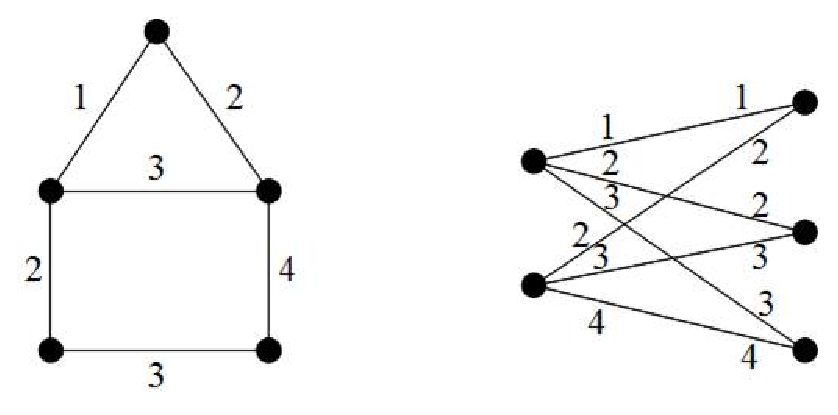
\includegraphics[width=20pc]{figures/W-bound-fig1.eps}\\
\caption{$3$ առավելագույն աստիճանով գրաֆներ, որոնք չունեն միջակայքային $3$-ներկում:}
\label{f1_cubic}
\end{center}
\end{figure}

Նկար \ref{f1_cubic}-ում պատկերված գրաֆները ցույց են տալիս, որ Թեորեմ \ref{t1_lower_matching_number}-ի ստորին գնահատականները հասանելի են: 

\begin{corollary}
\label{c1_lower_nopm} Եթե $G$ կապակցված մուլտիգրաֆը չունի կատարյալ զուգակցում և $G\in \mathfrak{N}$, ապա
\begin{center}
$w(G)\geq \max\{\Delta(G),2\delta(G)\}$:
\end{center}
\end{corollary}



Վերջապես, ապացուցենք Հետևանք \ref{c1_lower_nopm}-ի անալոգը կենտ մուլտիգրաֆների համար: $G$ մուլտիգրաֆը կանվանենք կենտ մուլտիգրաֆ, եթե $G$-ի բոլոր գագաթների աստիճանները կենտ են:

\begin{theorem}
\label{t1_lower_odd} Եթե $G$-ն կապակցված կենտ մուլտիգրաֆ է, $\vert
E(G)\vert-\frac{\vert V(G)\vert}{2}$ թիվը կենտ է և $G\in \mathfrak{N}$,
ապա
\begin{center}
$w(G)\geq \max\{\Delta(G),2\delta(G)\}$:
\end{center}
\end{theorem}
\begin{proof}[Ապացույց] Նշանակենք $\delta=\delta(G)$: Եթե $G$-ն չունի կատարյալ զուգակցում, ապա արդյունքը հետևում է Հետևանք \ref{c1_lower_nopm}-ից: Ենթադրենք $G$-ն ունի կատարյալ զուգակցում: Այժմ կատարենք հակասող ենթադրություն, դիցուք $G$-ն ունի $\alpha$ միջակայքային $t$-ներկում որևէ $t\leq 2\delta-1$ թվի համար: Քանի որ ցանկացած $v\in V(G)$, $1\leq \underline S\left(v,\alpha \right)\leq
\delta$, ստանում ենք, որ $\delta\in 
S_{\cap}\left(V(G),\alpha\right)$: Այստեղից հետևում է, որ $\delta$ գույնով ներկված կողերը $G$-ում կազմում են կատարյալ զուգակցում: Նշանակենք այդ կատարյալ զուգակցումը $M$-ով և դիտարկենք $G-M$ մուլտիգրաֆը: Սահմանենք $G-M$-ի $\beta$ ներկումը հետևյալ կերպ. ցանկացած $e\in E(G-M)$ կողի համար
\begin{center}
$\beta\left(e\right)=\left\{
\begin{tabular}{ll}
$\alpha(e)$, & երբ $1\leq \alpha(e)\leq \delta -1$,\\
$\alpha(e)-1$, & երբ $\delta+1\leq \alpha(e)\leq t$.\\
\end{tabular}%
\right.$
\end{center}

\begin{figure}[h]
\begin{center}
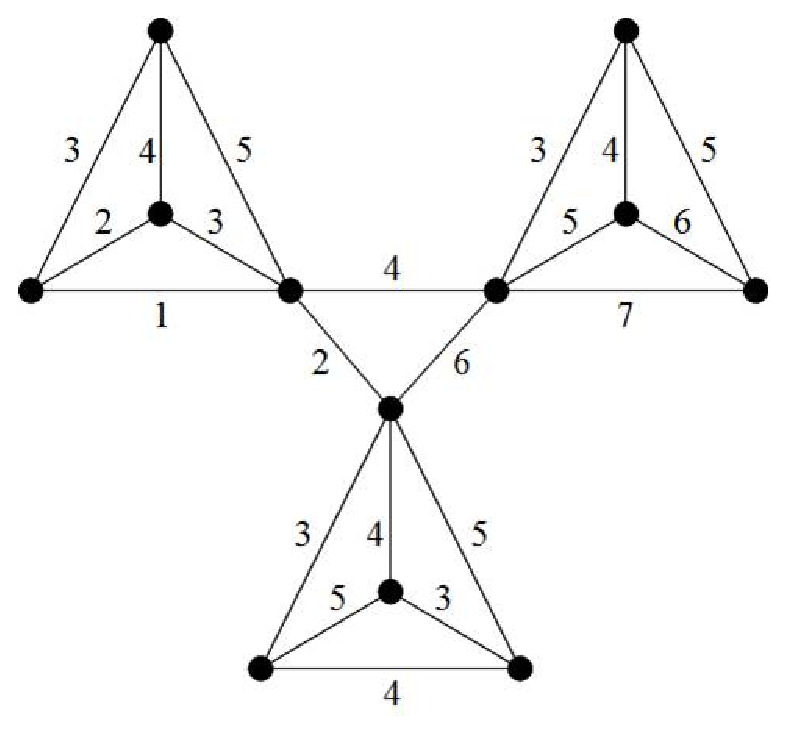
\includegraphics[width=20pc]{figures/W-bound-fig2.eps}\\
\caption{Միջակայքային ներկելի կապակցված գրաֆ $G$, որի բոլոր գագաթների աստիճանները կենտ են, $|E(G)|-\frac{|V(G)|}{2}=15$ և $w(G) \geq 6$:}
\label{f1_odd}
\end{center}
\end{figure}

Դժվար չէ տեսնել, որ $\beta$-ն $G-M$-ի միջակայքային $(t-1)$-ներկում է: Քանի որ $\vert E(G)\vert-\frac{\vert V(G)\vert}{2}$ կենտ է, ստանում ենք, որ $G-M$-ը զույգ մուլտիգրաֆ է կենտ թվով կողերով: Այստեղից հետևում է, որ $G-M$-ը ունի կենտ թվով կողեր պարունակող էյլերյան կապակցված բաղադրիչ, որը միջակայքային ներկելի է, ինչը հակասում է Հետևանք \ref{c1_eulerian}-ին:
\end{proof}